\section{Introduction}
A grid map is a discretisation of an enviroment into regular-sized cells known as \emph{tiles}
where each tile is connected with up 4 or 8 neighbours, depending on whether diagonal movement
is allowed or not.
In this paper we study the theoretical properties of 4-connected grid maps which appear frequently 
in the literature \cite{yap,swamps,far} and are often found in the pathfinding systems of modern 
video games.
For example, Square Enix's \emph{Heroes of Mana} (which appears on the Nintendo DS),
Astraware's \emph{My Little Tank} (iPhone) and Atari's \emph{Dragon Ball Z: Legacy of Goku} 
(Gameboy Advance) all make use of 4-connected grid maps for pathfinding and as a central
gameplay mechanic during combat.
\par
In the context of single-agent path finding A* \cite{hart68} is regarded as 
the gold standard search algorithm.
It is complete, optimal and optimally efficient which makes it very attractive 
to researchers in the area.
Many studies exist which have attempted to improve on the performance of A*. 
The majority focus in one of two directions: reducing the search space through hierarchical 
decomposition and identifying better heuristics to guide search. 
\par
In the case of hierarchical decomposition, techniques such as
HPA*~\cite{botea04} and PRA*~\cite{sturtevant05} seek to construct and explore
a much reduced approximate state space.
This makes them very fast. 
They also require no significant extra-memory when compared to A*.
However, they have the disadvantage that solutions are not guaranteed to be optimal.
\par
In case of the improved heuristics, it has been frequently shown
that obtaining better informed results than than the popular
Manhattan heuristic usually incurs significant memory overhead 
\cite{goldberg05,Cazenave:06,bjornsson06}.
Furthermore it is well known that even heuristics which differ from perfect information 
by at most a (small) additive constant, can still exhibit poor performance on a range of 
problems such as AI planning and path finding \cite{helmert08,pohl77}.
%Our simple example shown in Figure \ref{fig-emptymap}, which we discuss later,
%shows a similar behaviour in path finding.
\par
%When compared to a standard pathfinding method, such as A* with a Manhattan heuristic,
%all techniques outlined so far involve some kind of performance trade-off.
%They are typically faster than A* but, at the same time, require significant
%extra memory or provide no optimality guarantees.
In this work we explore a new speedup technique that aims to reduce the size of the search 
space while preserving optimality.
Our work is specific to 4-connected grid maps which allow straight but not diagonal movement.
We study this domain as it is highly symmetric, appears frequently in the literature 
\cite{yap,swamps,far} and is often found in the pathfinding systems of modern video games.
For example, Square Enix's \emph{Heroes of Mana} (which appears on the Nintendo DS),
Astraware's \emph{My Little Tank} (iPhone) and Atari's \emph{Dragon Ball Z: Legacy of Goku} 
(Gameboy Advance) all make use of 4-connected grid maps for pathfinding and as a central
gameplay mechanic during combat.
\par

Our work is inspired by hierarchical pathfinding systems such as HPA* \cite{botea04} but also shares
commonalities with symmetry elimination techniques that are used used to speed up search in areas 
such as constraint programming \cite{walsh}.

%%%%%
%Our work is based on the idea of symmetry elimination
%In this work we explore a technique called Optimal Hierarchical A* (OHA*) that 
%reduces the state space while preserving optimality.
%No significant additional memory is needed. 
%Infact, depending on the map topography, OHA* can use significantly less memory than standard A*.
%Furthermore, OHA* is shown to be on average between 1.7 to 3.3 
%times faster than A* on a large set of realistic maps.
%%%%%%


%OHA* is orthogonal to memory-intensive heuristics.
%The former reduces the size of the search graph before a search begins.
%The latter guide the exploration of the search graph.
%If desired, the two can be combined.

%\par
\par
%OHA* exploits the fact that in this domain there can be many equivalent 
%shortest path fragments between two locations on a map.
%In particular, OHA* seeks to reduce this number to just a few by identifying
%areas where equivalences exist and pruning away the majority of contributing nodes.
%This can reduce the search effort significantly, while still maintaining solution optimality.
%\par
% DDH: we discuss the approach in more detail toward the end. Does it add anything to do so here also?
%OHA* exploits the fact that there can be many shortest path fragments between two given location
%on an empty area of a map.
%Among many equivalent shortest fragments between two locations that belong to an optimal path,
%it is enough to consider one.
%This can reduce the search effort significantly, while maintaining solution optimality.

As a motivating example, consider Figure \ref{fig-emptymap} which requires
finding a shortest path from one room to another.
\begin{figure}[htbp]
       \begin{center}
                       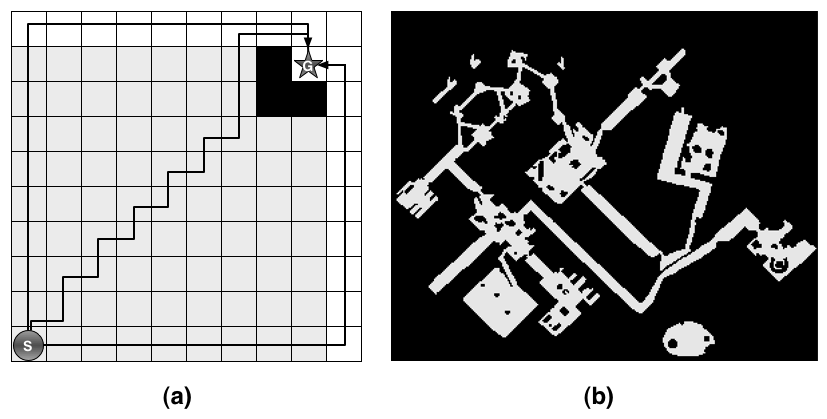
\includegraphics[scale=0.50, trim = 10mm 10mm 10mm 0mm]{diagrams/emptymap.png}
       \end{center}
	\vspace{-3pt}
       \caption{\textbf{(a)} A pathfinding instance that is simple to humans but difficult for a computer. 
				Many solutions exist; we highlight three. }
       \label{fig-emptymap}
\end{figure}
This scenario appears often in video games; for examples 
in video games.
%This simple domain appears in application areas such as robotics and \cite{latombe91} and video games
For example, BioWare's popular fantasy role-playing game \emph{Baldur's Gate} features complex dungeon
 areas that are composed of adjacent mostly empty rooms (see Figure \ref{fig-bgmap} for an example).
It can easily be shown that, in the example from Figure \ref{fig-emptymap}, the Manhattan heuristic is almost perfect: $\forall n, 0 \leq h^*(n) - h(n) \leq 2$.
Yet, if we apply A* to solving the instance in Figure \ref{fig-emptymap}, 
we find that every node in the grey area has an $f$-value smaller than the $f$-value of the target.
This means A* will necessarily expand them all. 
Given an unfavourable tie-breaking strategy A* will generate all nodes on the map and of those expand 
all but one.
\par
In solving the problem from Figure \ref{fig-emptymap} we observe that,
while many optimal-length solutions exist, there is no need to explore all of them.
In particular, either of the two solutions that go along the border of the map will do.
We generalise this observation to the related problem of traversing across empty rooms (which are 
often just as difficult for A* to solve) and show that it is possible to optimally navigate across 
such areas without ever exploring tiles that are not on the perimeter.
This result forms the basis OHA*, a new hierarchical pathfinding algorithm which 
decomposes 4-connected grid maps into a set of adjacent empty rooms.
We show that it is possible to optimally traverse an empty rectangular area by only ever expanding nodes along the perimeter of an empty room without ever needing to explore the interior.
To preserve optimality, macro-edges that traverse an empty rectangle in one step are added to some of the perimeter nodes. 
At the same time, regular edges to interior nodes are removed.
Overall, the branching factor of OHA* never increases as compared to standard A* on a grid map.
\par
OHA* is easy to understand and to implement. It can equivalently be seen either as
a standard A* run on a search graph slightly different than a standard grid, or
as a slightly modified A*, with a different successor generation rule,
run on a standard grid state space.
\par
We undertake an empirical analysis and show that our technique is also fast and memory efficient.
Thus, unlike most pathfinding techniques on grid maps, OHA* is able to provide a speed-up over A*
without compromising other important performance criteria, such as the memory requirements
and the optimality of solutions.

The rest of the paper is structured as follows.
Next we overview related work.
Section \ref{algorithm} describes OHA*, our pathfinding algorithm.
Decomposing the traversable part of a grid map into a partition of empty areas,
which is required by OHA*, is the topic of Section~\ref{empty rooms}.
Then, we present our experiments and results.
The last section contains conclusions and future work ideas.

